%% img/NPClass/SATproof3.tex
%% Copyright 2019 Andrea Berlingieri
%
% This work may be distributed and/or modified under the
% conditions of the LaTeX Project Public License, either version 1.3
% of this license or (at your option) any later version.
% The latest version of this license is in
%   http://www.latex-project.org/lppl.txt
% and version 1.3 or later is part of all distributions of LaTeX
% version 2005/12/01 or later.
%
% This work has the LPPL maintenance status `maintained'.
%
% The Current Maintainer of this work is Andrea Berlingieri.
%
% This work consists of all files listed in manifest.txt
\documentclass{standalone}

\usepackage{../TikzStyle}
\usepackage{../mystyle}
\usetikzlibrary{calc}
\usetikzlibrary{patterns}

\newcommand{\Row}[3]{% x,y,length
    \draw[xshift=#1 cm,yshift=#2 cm] (0,0) -- (#3,0);
    \draw[xshift=#1 cm,yshift=#2 cm] (0,0) -- (0,-0.75);
    \draw[xshift=#1 cm,yshift=#2 cm] (0,-0.75) -- (#3,-0.75);
    \draw[xshift=#1 cm,yshift=#2 cm] (#3,0) -- (#3,-0.75);
%    \node () at ([shift={(#1,0)}]0.7,-0.5) {$\textit{nome}_{#2}$};
}

\newcommand{\Column}[3]{% x,y,height
    \draw[xshift=#1 cm,yshift=#2 cm] (0,0) -- (0,-#3);
    \draw[xshift=#1 cm,yshift=#2 cm] (0,0) -- (0.75,0);
    \draw[xshift=#1 cm,yshift=#2 cm] (0.75,0) -- (0.75,-#3);
    \draw[xshift=#1 cm,yshift=#2 cm] (0,-#3) -- (0.75,-#3);
%    \node () at ([shift={(#1,0)}]0.7,-0.5) {$\textit{nome}_{#2}$};
}

\newcommand{\Cell}[3]{% tlcx,tlcy,content (tlc=top left corner)
    \draw[xshift=#1 cm,yshift=#2 cm] (0,0) -- (0.75,0);
    \draw[xshift=#1 cm,yshift=#2 cm] (0,-0.75) -- (0.75,-0.75);
    \draw[xshift=#1 cm,yshift=#2 cm] (0,0) -- (0,-0.75);
    \draw[xshift=#1 cm,yshift=#2 cm] (0.75,0) -- (0.75,-0.75);
    \node () at ([shift={(#1,#2)}]0.375,-0.375) {#3}
%    \node () at ([shift={(#1,0)}]0.7,-0.5) {$\textit{nome}_{#2}$};
}

\newcommand{\BCell}[4]{% tlcx,tlcy,content,length (tlc=top left corner)
    \draw[xshift=#1 cm,yshift=#2 cm] (0,0) -- (#4,0);
    \draw[xshift=#1 cm,yshift=#2 cm] (0,-0.75) -- (#4,-0.75);
    \draw[xshift=#1 cm,yshift=#2 cm] (0,0) -- (0,-0.75);
    \draw[xshift=#1 cm,yshift=#2 cm] (#4,0) -- (#4,-0.75);
    \node () at ([shift={(#1,#2)}]$(0,0)!0.5!(#4,-0.75)$) {#3}
%    \node () at ([shift={(#1,0)}]0.7,-0.5) {$\textit{nome}_{#2}$};
}

\begin{document}
    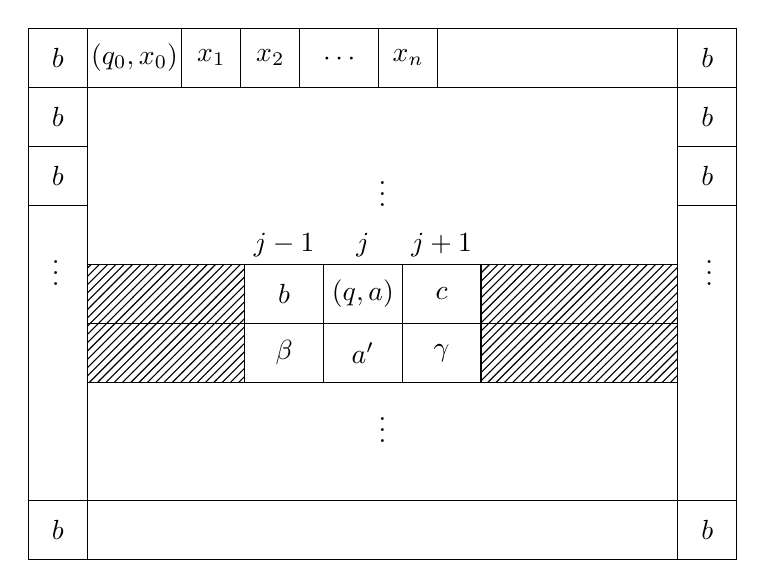
\begin{tikzpicture}
        \Row{0.5}{0}{7.5};
        \Row{0.5}{-6}{7.5};
        \Column{-0.25}{0}{6.75};
        \Column{8}{0}{6.75};

        \BCell{0.5}{0}{$(q_{0},x_{0})$}{1.2};
        \Cell{1.7}{0}{$x_{1}$};
        \Cell{2.45}{0}{$x_{2}$};
        \node () at (3.7,-0.4) {$\cdots$};
        \Cell{4.2}{0}{$x_{n}$};

        \Row{0.5}{-3}{7.5};
        \Row{0.5}{-3.75}{7.5};
        \BCell{2.5}{-3}{$b$}{1};
        \BCell{2.5}{-3.75}{$\beta$}{1};
        \BCell{3.5}{-3}{$(q,a)$}{1};
        \BCell{3.5}{-3.75}{$a'$}{1};
        \BCell{4.5}{-3}{$c$}{1};
        \BCell{4.5}{-3.75}{$\gamma$}{1};
        \node () at (4.25,-2) {$\vdots$};
        \node () at (4.25,-5) {$\vdots$};

        \draw[pattern=north east lines,pattern color=black] (0.5,-3) rectangle (2.5,-3.75);
        \draw[pattern=north east lines,pattern color=black] (0.5,-3.75) rectangle (2.5,-4.5);

        \draw[pattern=north east lines,pattern color=black] (5.5,-3) rectangle (8,-3.75);
        \draw[pattern=north east lines,pattern color=black] (5.5,-3.75) rectangle (8,-4.5);

        \node () at (3,-2.75) {$j-1$};
        \node () at (4,-2.75) {$j$};
        \node () at (5,-2.75) {$j+1$};

        \Cell{-0.25}{0}{$b$};
        \Cell{-0.25}{-0.75}{$b$};
        \Cell{-0.25}{-1.5}{$b$};
        \node () at (0.1,-3) {$\vdots$};
        \Cell{-0.25}{-6}{$b$};

        \Cell{8}{0}{$b$};
        \Cell{8}{-0.75}{$b$};
        \Cell{8}{-1.5}{$b$};
        \node () at (8.4,-3) {$\vdots$};
        \Cell{8}{-6}{$b$};


    \end{tikzpicture}
\end{document}
